\chapter{Cryptography techniques}
Cryptography is a mathematical technique that permits to transmit the data to a form that can't be understood by unauthorized users.
\begin{figure}[H]
    \centering
    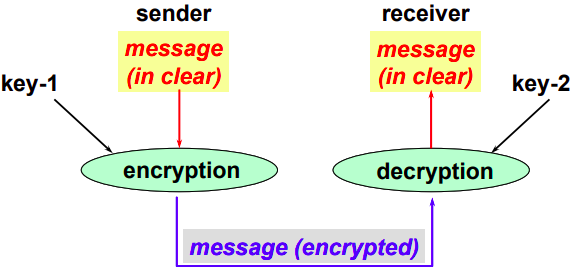
\includegraphics[width=0.5\textwidth]{/home/lorenzo/Notes/Information System Security/images/image copy 13.png}
\end{figure}
\noindent
To explain the various concepts of cryptography we need to introduce some terminology:
\begin{itemize}
    \item \textbf{Plaintext (P)}: the original message before encryption.
    \item \textbf{Ciphertext (C)}: the encrypted message that appears scrambled.
\end{itemize}
\begin{quotebox-grey}{Kerckhoffs' Principle}
\begin{minipage}{0.7\textwidth}
	\vspace{-0.3cm}
This principle states that the security of a cryptographic system should rely on the \textbf{secrecy of the keys}, not the secrecy of the encryption algorithm itself. 
If the keys:
\begin{itemize}
\item are kept secure, this ensures only authorized parties can decrypt the message.
\item are managed by trusted systems, this minimizes the risk of unauthorized access.
\item are of adequate length, they are harder to crack with brute force methods. 
\end{itemize} 
\end{minipage} 
\hspace{0.3cm}
\begin{minipage}{0.3\textwidth}
    \centering
    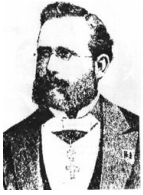
\includegraphics[width=0.4\textwidth]{/home/lorenzo/Notes/Information System Security/images/image copy 14.png}
\end{minipage}
\noindent
\\
\\
\textbf{It's no important that the encryption and decryption algorithms are kept secret}, on the contrary it's better to make the algorithms public so that they can be widely analysed and their possible weakness identified. 
\\
\\
Kerchoff’s Principle is tightly correlated to the principle of \textbf{Security Through Obscurity
(STO)}: a system is protected but the details on how it has been protected are not disclosed.
This alone is not considered a valid security mechanism. STO can be used as a layer of the security system \textbf{only if} a really strong algorithm is used
\end{quotebox-grey}
\newpage
\section{Symmetric Cryptography}
\textbf{Symmetric cryptography} is so called because it uses \textbf{only} a single key \textbf{shared between} the sender and the receiver. 
\[key1=key2=K\]
The key \textbf{K} is used to generate the Ciphertext \textbf{C} by encrypting the Plaintext \textbf{P}. \textbf{C} is then sent to the receiver, which recovers \textbf{P} by applying the decryption algorithm using \textbf{K}:
\[C\ =\ enc(K,P)\ =\ \{P\}K\]
\[P\ =\ dec(K,C)\ =\ enc^{-1}(K,C)\]
\begin{figure}[H]
    \centering
    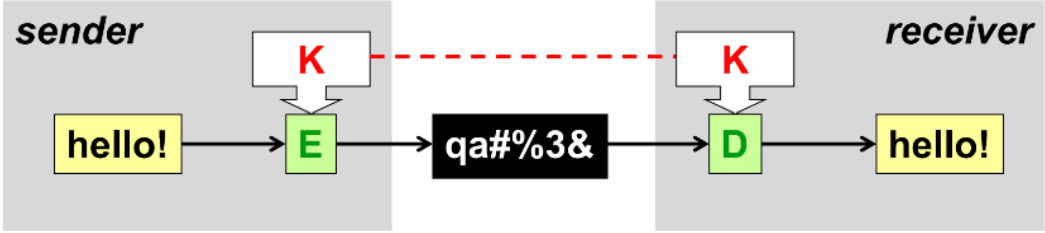
\includegraphics[width=0.5\textwidth]{/home/lorenzo/Notes/Information System Security/images/Screenshot from 2024-12-27 13-04-27.png}
\end{figure}
\noindent
\textbf{Symmetric Encryption} requires the use of a unique \textbf{K} for each peer couple. A complete pairwise private communication between N parties would requires:
 \[\frac{N \cdot (N-1)}{2}\ \text{unique \textbf{K}s}\]
The parties can exchanged \textbf{securely} the \textbf{K}s in two ways:
\begin{itemize}
    \item \textbf{OOB} (\textbf{Out-Of-Band}): the parties share the \textbf{K} without using electronic channel used for transmitting the encrypted message.
    \item \textbf{Key Exchange Algorithms}: algorithms such as Diffie-Helmann enable parties to securely exchange keys over a potentially insecure channel.
    \begin{figure}[H]
        \centering
        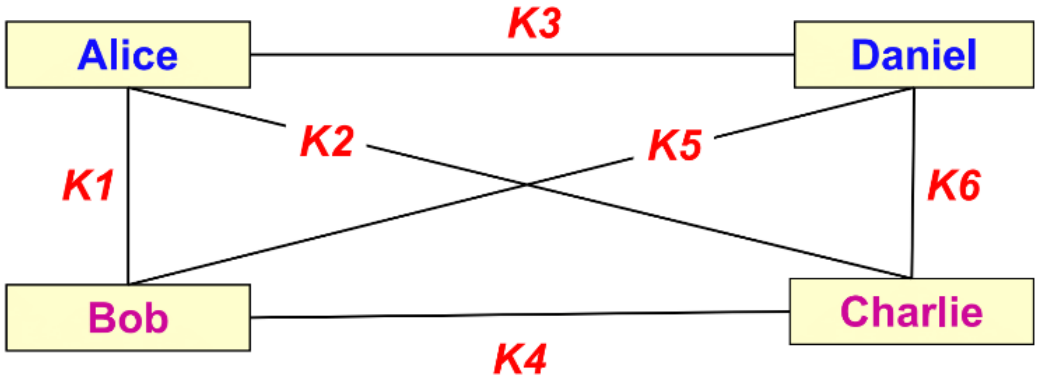
\includegraphics[width=0.4\textwidth]{/home/lorenzo/Notes/Information System Security/images/Screenshot from 2024-12-27 15-26-15.png}
    \end{figure}   
\end{itemize}
\begin{quotebox-grey}{Symmetric Block Encryption Algorithms}
    The main type of symmetric is the \textbf{Block Algorithm}. Each algorithm elaborates encryption/decryption \textbf{only if} a minimum amount of data  (typically 64/128 bits) is available.
    \vspace{0.2cm}
        \begin{center}
            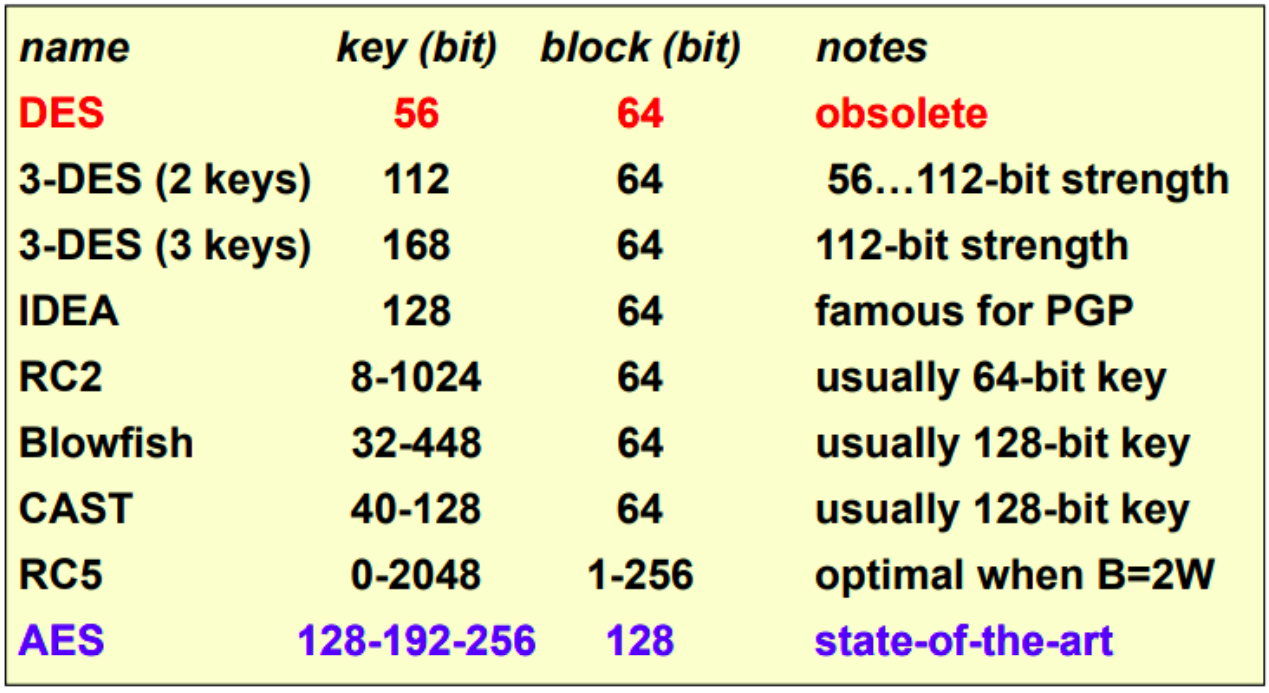
\includegraphics[width=0.5\textwidth]{/home/lorenzo/Notes/Information System Security/images/Screenshot from 2024-12-27 15-57-24.png}
        \end{center}
\end{quotebox-grey}

\newpage
\subsection{DES (Data Encryption Standard)}
DES uses \textbf{64 bits keys}, yet its effectiveness is only the one of a 56 bits key, since 8 bits of the key are used to check the parity of the others. This means that, when DES generates a key, every 7 bits that are generated, another is added to check the parity of the previous 7 bits. It's designed to be \textbf{efficient in hardware} because it requires: 
\begin{itemize}
    \item \textbf{XOR in details}: elementary operation on all the CPUs.
    \begin{quotebox}[colframe=blue!10!white, colback=blue!5!white]{XOR}
        It's a fundamental operation in cryptography, it provides "confusion" by randomizing input data.
        ruth table:
        \begin{center}
        \begin{tabular}{|c|c|c|}

\hline
A & B & A XOR B \\
\hline
0 & 0 & 0 \\
0 & 1 & 1 \\
1 & 0 & 1 \\
1 & 1 & 0 \\
\hline
\end{tabular}
\end{center}

Notes that it's the \textbf{inverse of itself}:
\begin{itemize}
    \item if \(A\ xor\ B\ =\ Z\) then \(Z\ xor\ B\ =\ A\) (or \(Z\ xor\ A\ =\ B\))
\end{itemize}
    \end{quotebox}
    \item \textbf{Shift}: elementary operation on all the CPUs.
    \item \textbf{Permutation}: expensive operation  yet efficient if done directly in hardware.
    \begin{figure}[H]
        \centering
        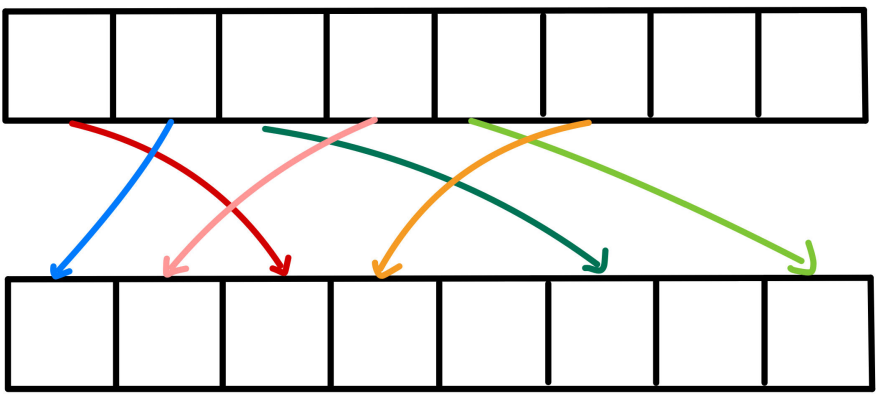
\includegraphics[width=0.3\textwidth]{/home/lorenzo/Notes/Information System Security/images/Screenshot from 2024-12-27 15-56-26.png}
    \end{figure}
\end{itemize}

\subsection{3-DES or Triple DES}
It was introduced as an improved version of the original DES. It is simply the repeated application of the DES. It uses \textbf{two} or \textbf{tree} keys. Usually, 3-DES is applied in the \textbf{EDE} (\textbf{Encryption-Decryption-Encryption}) \textbf{mode}:
\begin{itemize}
    \item \textbf{With 2 keys} \(\rightarrow \) Uses two 56-bit keys (K1 and K2), repeating K1 for the
    third operation:
    \[C'\ =\ enc(K_1,P)\ \ \ C''=dec(K_2,C')\ \ \ C=enc(K_1,C'')\]
    \begin{quotebox-red}{Beware}
        If sufficient memory is available for attack (about \(2^{59} B\)), the effective security
        of this scheme is roughly \textbf{56 bits}, due to vulnerabilities. Without that much
        memory, the effective key size is \textbf{12 bits}.
    \end{quotebox-red}
    \item \textbf{With 3 keys} \(\rightarrow \) Uses three distinct keys (K1, K2, and K3), providing better security with an effective key size of 112 bits:
    \[C'\ =\ enc(K_1,P)\ \ \ C''=dec(K_2,C')\ \ \ C=enc(K_3,C'')\]
\end{itemize}
\begin{customquote}
\vspace{-0.4cm}
\subsubsection{Why 2-DES is not used?}
Because the double application of any encryption algorithm is subject to a \textbf{Known-Plaintext Attack}, which is a kind of MIMT attack. This attack allows to decrypt data with \textbf{at most \(2^{N+1}\)} attempts (if the keys are N-bit long).
\\
\\
During a Known-Plaintext attack both \textbf{P} and \textbf{C} (\(=enc(K_2,enc(K_1,P))\) are \textbf{sniffed by} the attacker. Hypothesizing N bits keys, the attacker can then compute \textbf{K} by:
\begin{enumerate}
    \item Compute \(2^N\) values \(X_i=enc(K_i,P)\)
    \item Compute \(2^N\) values \(Y_j=dec(K_j,C)\)
    \item Search of those values \(K_i\) and \(K_j\) such that \(X_i=Y_j\)
    \item Discard false positive
\end{enumerate}
\end{customquote}


\subsection{AES (Advanced Encryption Standard))}
AES was established through a public international competition aimed at replacing the Data Encryption Standard (DES). On October 2, 2000, Rijndael was selected as the winner of the AES competition, featuring:
\begin{itemize}
    \item Key lengths of 128, 192, or 256 bits.
    \item A block size of 128 bits.
    \item Officially published in November 2001 as FIPS-197.
    \item Gradual adoption after 2010, as cryptographic algorithms need time to prove their reliability.
\end{itemize}

\subsection{Application Modes for block algorithms}
Block algorithms are designed to encrypt \textbf{fixed-size} blocks of data, so when dealing with data of varying lengths, specific techniques must be applied:
\begin{itemize}
    \item \underline{\textbf{Size of Data to Encrypt > Algorithm's Block Size}}
    \begin{itemize}
        \item \textbf{ECB (Electronic Code Block)}: In ECB mode, each block of plaintext is encrypted independently of the others, which makes the encryption formula for the n-th block as follows:
        \[C_n=enc(K,P_n)\]
        In this mode, \textbf{decryption} is the reverse of the encryption process. The formula for decrypting the n-th block is as follows:
        \[P_n=enc^{-1}(K,C_n)\]
        Since there is no dependency between blocks, an error in transmission of one block generates an error at the decryption of only the affected block.
        \begin{figure}[H]
            \centering
            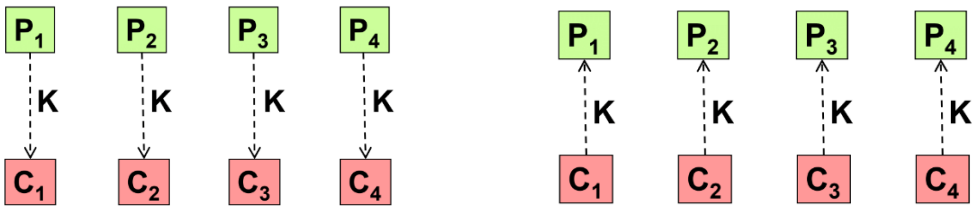
\includegraphics[width=0.7\textwidth]{/home/lorenzo/Notes/Information System Security/images/Screenshot from 2024-12-27 17-23-56.png}
        \end{figure}

        \begin{quotebox-red}{Problems with ECB mode}
            \begin{itemize}
            \item \underline{Swapping of ciphertext blocks goes undetected}: since each block is encrypted independently, if two ciphertext blocks are swapped, the decrypted message will still be valid but with blocks in the wrong order. 
            \item \underline{Identical plaintext blocks generate identical ciphertext blocks}: when two plaintext blocks are the same, their corresponding ciphertext blocks will also be identical. This lack of variation reveals patterns in the data, making it vulnerable to known-plaintext attacks 
        \end{itemize}
        \end{quotebox-red}
        \textcolor{red}{\textbf{N.B.}} \textbf{Parallel encryption and decryption are possible} because ECB blocks are independent from each other. 
        \vspace{0.1cm}
        \item \textbf{CBC (Cipher Block Chaining)}: In CBC mode, each plaintext block is XORed with the previous ciphertext block before being encrypted. The formula for encrypting the n-th block is:
        \[C_n=enc(K,P_n \oplus C_{n-1})\]
        The first plaintext block is XORed with the \textbf{IV} (\textbf{Initialization vector}) instead of a previous ciphertext block because no previous ciphertext exists for the first block. The  \textbf{IV} should be \textbf{random and unique} for every  \textbf{encryption} session.\\ 
        The \textbf{decryption} process involves reversing the encryption steps:
        \begin{figure}[h]
            \centering
            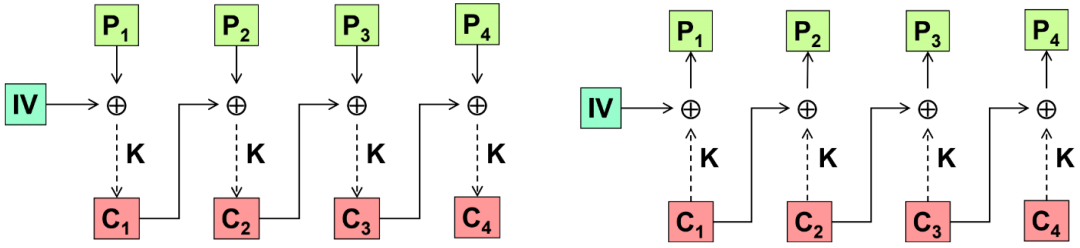
\includegraphics[width=0.8\textwidth]{/home/lorenzo/Notes/Information System Security/images/Screenshot from 2024-12-27 17-38-40.png}
        \end{figure}
        \begin{quotebox-red}{Problems with CBC mode}
            A single  error in a ciphertext block affects only two plaintext blocks:
            \begin{enumerate}
                \item The block corresponding to the erroneous ciphertext block.
                \item The next block.
            \end{enumerate}
        \end{quotebox-red}
        \textcolor{red}{\textbf{N.B.}} CBC allows for \textbf{parallel decryption} but not \textbf{parallel encryption}.
        \end{itemize}
    
    
\item \underline{\textbf{Size of data Encrypt < Algorithm's Block Size}} 
\begin{itemize}
    \item \textbf{Padding}: Padding is used to \textbf{fill the only last block} until it reaches the required block size (\textbf{C} will be longer than \textbf{P}).
    \begin{figure}[H]
        \centering
        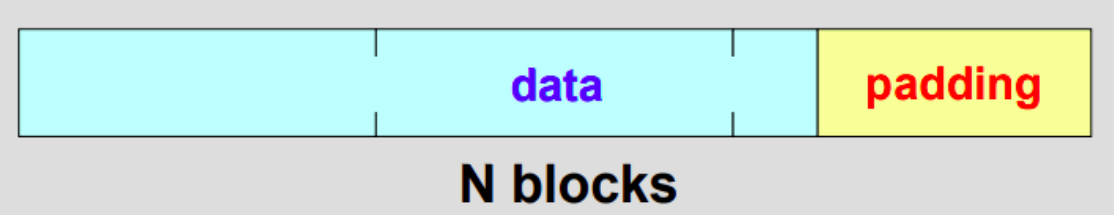
\includegraphics[width=0.5\textwidth]{/home/lorenzo/Notes/Information System Security/images/Screenshot from 2024-12-27 18-09-09.png}
    \end{figure}
    Depending on the chosen \textbf{Padding Technique}, we can allow or avoid different kind of attacks. Some techniques also offer minimal integrity control (e.g. if the key is wrong or data is manipulated, the padding bytes are incoherent).When the data size is smaller than the block size, special techniques such as \textbf{CFB} (\textbf{Cipher FeedBack}) or \textbf{OFB} (\textbf{Output FeedBack}) are the preferred.\\
    Even if the plaintext is an exact multiple of the block size, padding must still be added to avoid errors in the interpretation of the last block. 
    \vspace{0.1cm}
    \item \textbf{CTS (Ciphertext Stealing)}: CTS allows the use of block algorithms \textbf{without} the need of Padding. CTS works in the following way:
    \begin{enumerate}
        \item The last (partial block) \(P_N\) is filled with a copy of the last bytes taken from the penultimate block \(P_{N-1}\).
        \item The copied bytes are \textbf{removed} form the (now partial) penultimate block.
        \item After encryption, the last and penultimate block' positions are \textbf{exchanged}.
    \end{enumerate}
    \begin{figure}[H]
        \centering
        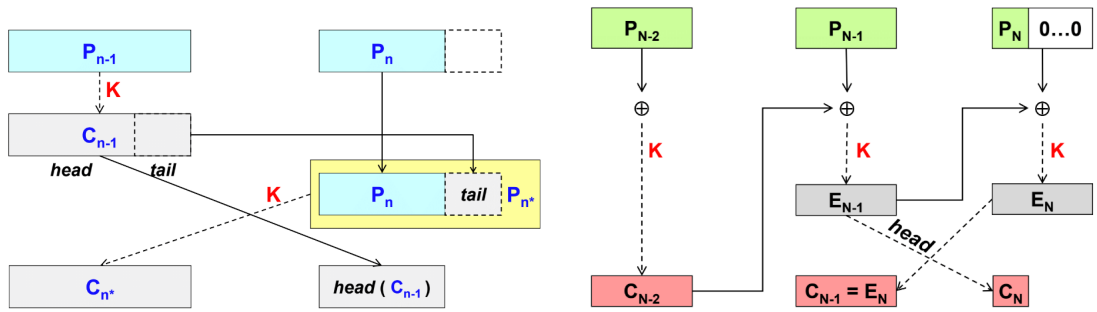
\includegraphics[width=0.7\textwidth]{/home/lorenzo/Notes/Information System Security/images/image copy 15.png}   
    \end{figure}
    \textcolor{red}{\textbf{N.B.}} CTS is particularly useful when we cannot increase the size of the data after encryption, such as in storage encryption. The computation time of encryption slightly increases due to the need for additional steps, such as modifying and swapping blocks.
    \vspace{0.1cm}
    \item \textbf{CTR (Counter Mode)}: CTR modifies block algorithm in order to encipher N bits at a time (often N = 1). CTR can be used \textbf{only} to encipher \textbf{P} smaller than one block size. It does not require padding and allows random direct access to any ciphertext block (no dependency between blocks). Requires a \textbf{nonce} and a \textbf{counter}, combined by a suitable function (concatenation, XOR, etc.) to generate the input block. CTR works in the following way:
    \begin{enumerate}
        \item \textbf{f(nonce, counter)} outputs exactly one block size of data.
        \item This block gets encrypted with the \textbf{K}.
        \item The \textbf{leftmost group} (meaning the first N bits) are extrapolated from the block and are \textbf{XOR}ed with the corresponding \(P_i\)’s group, which in turn generates the corresponding \(C_i\)’s group.
    \end{enumerate}
    \begin{figure}[H]
        \centering
        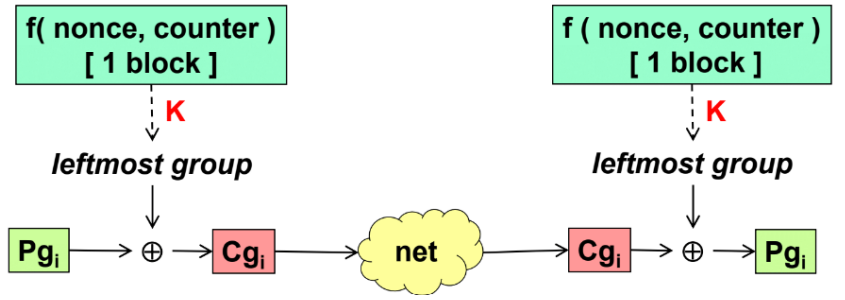
\includegraphics[width=0.7\textwidth]{/home/lorenzo/Notes/Information System Security/images/image copy 16.png}
    \end{figure}
    \begin{quotebox-red}{Cancellation attacks}
        CTR mode is vulnerable to cancellation attacks because it relies on synchronized counters between sender and receiver.    
    \end{quotebox-red}
    \begin{quotebox-yellow}{CTR as a stream ciphertext}
    The byte-oriented CTR mode of a block algorithm may be considered a stream algorithm.
    \end{quotebox-yellow}
    \textcolor{red}{\textbf{N.B.}} Moreover, if a group is \textbf{modified}, the error does not propagate to the successive group since group are independent \(\rightarrow \) it is possible to decrypt a random group \textbf{without} having decrypt the others.
    \\\textbf{Parallel encryption and decryption are possible.} 
\end{itemize}
\end{itemize}

\subsection{Stream Encryption Algorithms}
\begin{minipage}{0.6\textwidth}
%	\vspace{-0.5cm}
\textbf{Sream Encryption Algorithms} are another kind of Symmetric Encryption algorithms that \textbf{not} require the division of the \textbf{P} in blocks, as they tipically works with a \textbf{single} bit or byte at a time. This category contains the \textbf{only perfect algorithm} which is called \textbf{One-Time-Pad}: the algorithm requires a \textbf{K} as long as \textbf{P}, for this reason it's \textbf{not} of pratical use (unless \textbf{P} is very small).\\Real stream algorithms use \textbf{pseudo-random key generators}, which \textbf{must} be synchronized between sender and receiver. For example, \textbf{RC4} and \textbf{SEAL} are some \textbf{old}
instances of stream algorithms, while CTR can be considered a stram algorithm when \textbf{N=1}.
\end{minipage} 
\hspace{0.5cm}
\begin{minipage}{0.4\textwidth}
    \centering
    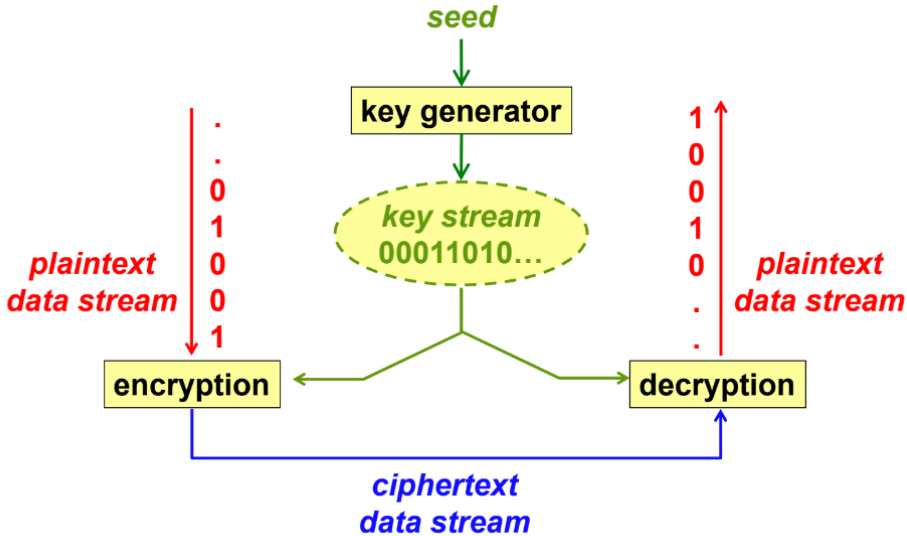
\includegraphics[width=\textwidth]{/home/lorenzo/Notes/Information System Security/images/Screenshot from 2024-12-28 11-20-36.png}
\end{minipage}



